\section{Experimentálne overenie funkčnosti riešenia} \label{sec:experimenty}

Táto kapitola je venovaná overeniu správnosti implementácie. Boli vykonané nasledujúce štyri experimenty, 
ktoré mali potvrdiť, alebo vyvrátiť správnu funkčnosť riešenia. 
\begin{enumerate}
 \item \textbf{Prvý test} overil konektivitu a prenos údajov medzi exportérom a mediátorom a následne medzi 
 mediátorom a kolektorom.
 \item \textbf{Druhý test} porovnal hodnoty údajov exportovaných BEEM-om s~hodnotami uloženými v~databáze po prechode
 cez Mediátor bez sprostredkovateľského procesu.
 \item \textbf{Tretí test} demonštroval správnosť anonymizácie údajov v~podaní sprostredkovateľského procesu 
 \verb|ExampleProcess|, spomínaného vyššie v~návrhu a implementácii.
 \item \textbf{Štvrtý test} bol tzv. záťažovým testom, overoval stabilitu Mediátora pri dlhodobom behu a 
 pri spracovávaní prevádzky s~vysokým počtom tokov.
\end{enumerate}

%%----------------------

\subsection{Testovacia topológia}

Pri prvých troch testoch bol použitý virtualizačný nástroj VirtualBox, v~ktorom boli vytvorené tri virtuálne 
počítače, zapojené do topológie, ktorú možno vidieť na Obrázku~\ref{o:test_topologia}.
Na všetkých troch počítačoch sa používal operačný systém \emph{Ubuntu 12.04 LTS} v~desktopovej verzii. Na 
prvom počítači bol nainštalovaný exportér BEEM (verzia 1.1-6 s~podporou pre IPFIX Mediátor), ktorý 
exportoval správy druhému počítaču na UDP port vyhradený pre IPFIX komunikáciu - \emph{4739}. Tam bežal 
Mediátor verzie 1.0. Ten zase preposielal správy na tretí počítač (taktiež port \emph{4739}), kde bol 
spustený JXColl (verzia 3.9) s~funkčnou PostgreSQL databázou. Počítače boli zapojené v~jednej 
lokálnej sieti a všetky mali prístup na Internet.

\begin{figure}[ht!]
\centering
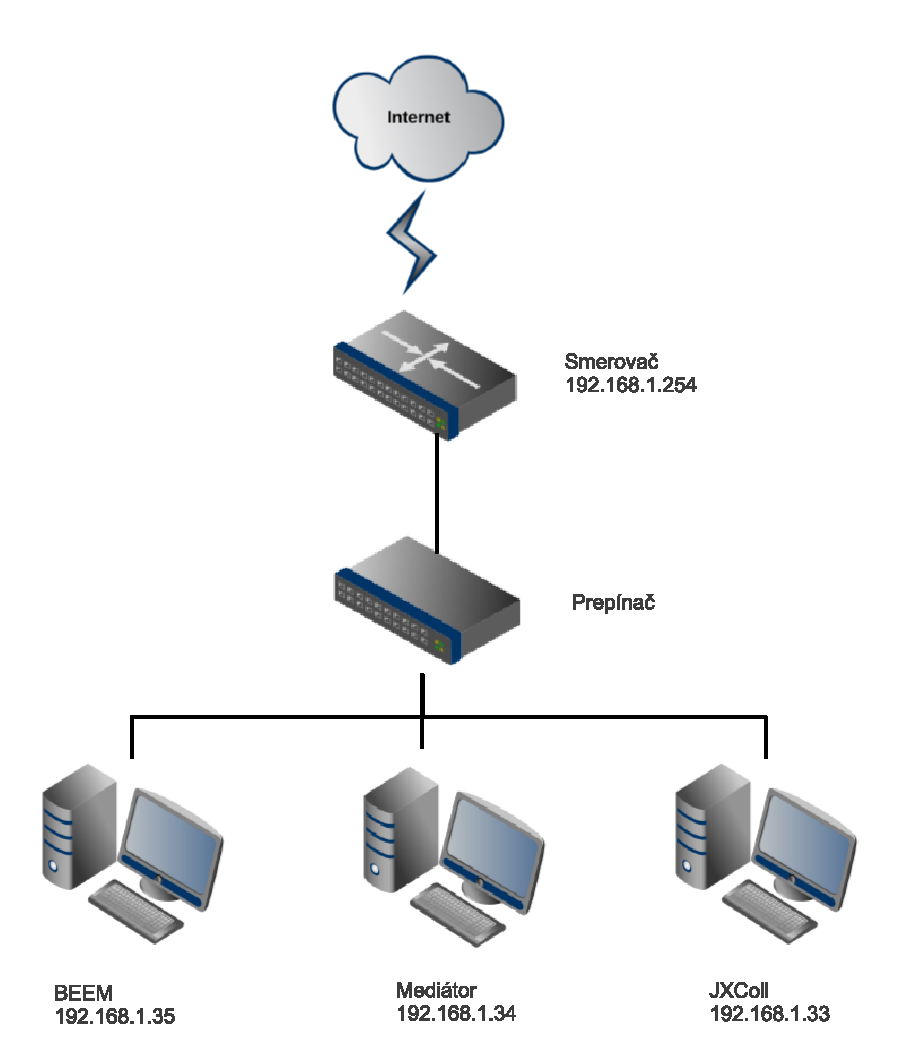
\includegraphics[width=0.8\textwidth]{test_topologia}
\caption{Testovacia topológia}\label{o:test_topologia}
\end{figure}

%%-------------------------

\subsection{Test konektivity}

Prvý experiment overoval základnú konektivitu medzi exportérom a kolektorom v~prípade, že je medzi ne 
zaradený mediátor. Vo svojej východiskovej konfigurácii vypisuje BEEM logovacie správy na štandardný 
výstup. Tie obsahujú základné informácie o~každom exportovanom zázname o~toku ako to môžeme vidieť na 
Obrázku~\ref{o:konektivita_beem}. Mediátor mal nastavenú úroveň logovacích výstupov na \emph{DEBUG}, 
čo zahŕňa nielen chybové hlášky, ale aj všetky informačné a ladiace oznamy. 

Konektivita medzi exportérom
a mediátorom bola potvrdená, na Obrázku~\ref{o:konektivita_mediator} je zachytený výstup Mediátora po 
prijatí správy od exportéra. Výpis obsahuje IP adresu a port z~ktorého prišla správa, jej veľkosť a 
oznam, že ide o~IPFIX správu. Za tým nasledujú hodnoty z~hlavičky správy a výpis všetkých sád, ktoré
správa obsahuje. Potom bol spracovaný záznam o~toku posunutý dispečerovi -- \verb|FlowRecordDispatcher|, 
ktorý ho poslal na export. Tam sa záznam o~toku naspať zabalil do nového IPFIX paketu a ten bol odoslaný 
smerom na kolektor.

\begin{figure}[ht!]
\centering
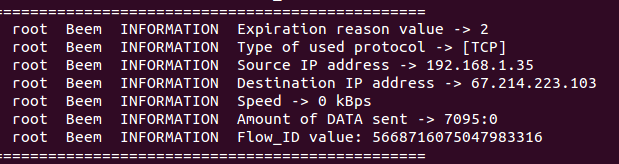
\includegraphics[width=0.9\textwidth]{konektivita_beem}
\caption{Test 1: Konektivita medzi exportérom a Mediátorom -- strana exportéra}\label{o:konektivita_beem}
\end{figure}

\begin{figure}[ht!]
\centering
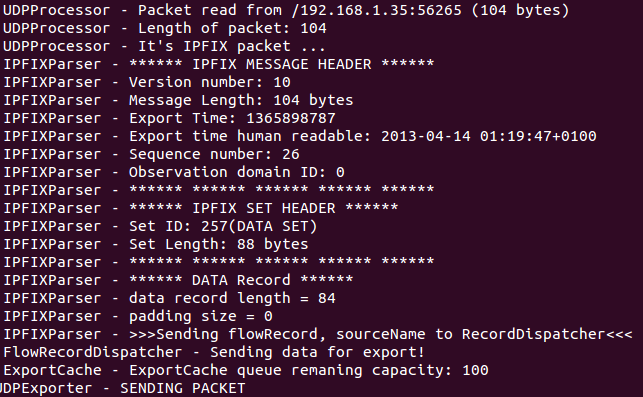
\includegraphics[width=0.9\textwidth]{konektivita_mediator}
\caption{Test 1: Konektivita medzi exportérom a Mediátorom -- strana Mediátora}\label{o:konektivita_mediator}
\end{figure}

Konektivita medzi Mediátorom a kolektorom bola tiež potvrdená. Dôkazom boli logovacie výstupy kolektora, 
ktoré sú veľmi podobné ako tie z~Mediátora. V~databáze, na ktorú je JXColl pripojený, pribúdali správne 
záznamy. Tento experiment môžeme považovať za úspešný.

%%-------------------------

\subsection{Test správnej reprezentácie údajov}

Druhý experiment nadväzoval na predchádzajúci test konektivity. Testovacia topológia aj konfigurácie 
jednotlivých nástrojov boli rovnaké ako v~predchádzajúcom prípade. V~Mediátore stále neboli spustené 
žiadne sprostredkovateľské moduly. 

Myšlienkou tohto overenia bolo porovnať dáta, ktoré posiela exportér s~dátami, ktoré prejdú celou topológiou
cez Mediátor a JXColl a sú uložené v~databáze. Na zachytenie správ z~BEEM-u bol použitý program 
Wireshark, ktorý odchytával sieťovú prevádzku na prvom počítači, na rozhraní \emph{eth0} s~IP adresou 
\emph{192.168.1.35}. Detail jednej zo správ, ktoré zachytil Wireshark je na Obrázku 
\ref{o:porovnanie_wireshark}. Na Obrázku \ref{o:porovnanie_db} sú zase vyfiltrované posledné záznamy, 
ktoré boli uložené do databázy. Môžeme porovnať aspoň na niekoľkých znázornených informačných elementoch,
že záznamy o~toku sa po prechode cez topológiu s~Mediátorom bez zapnutých sprostredkovateľských procesov 
nezmenili. Tento experiment považujeme za úspešný.

\begin{figure}[ht!]
\centering
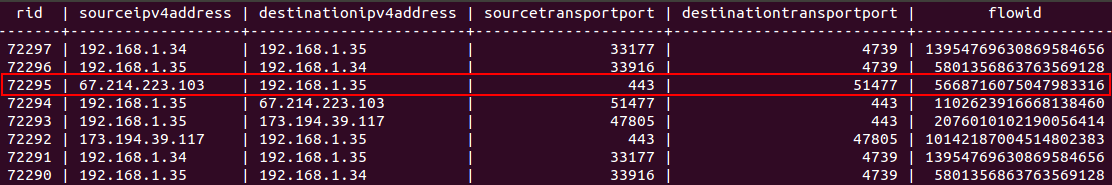
\includegraphics[width=1.0\textwidth]{porovnanie_db}
\caption{Test 2: Výpis obsahu databázy}\label{o:porovnanie_db}
\end{figure}

\begin{figure}[ht!]
\centering
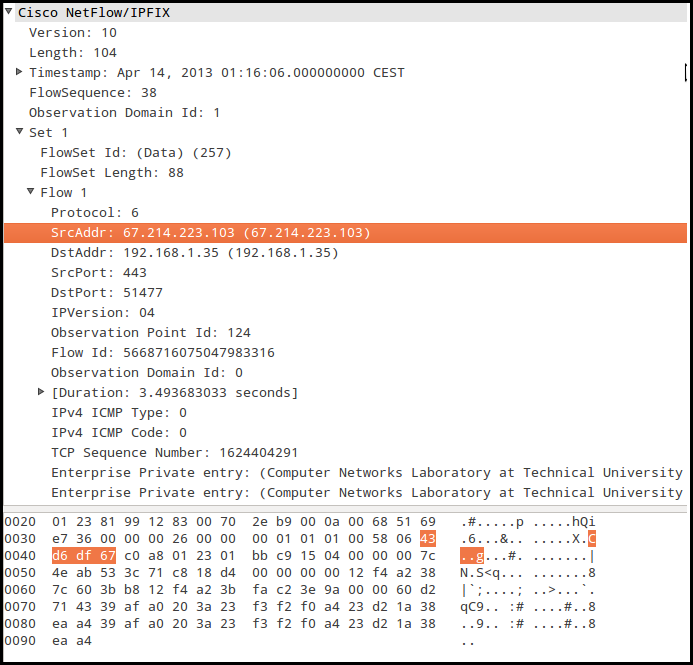
\includegraphics[width=1.0\textwidth]{porovnanie_wireshark}
\caption{Test 2: Správy odosielané exportérom zachytené programom Wireshark}\label{o:porovnanie_wireshark}
\end{figure}



%%-------------------------

\subsection{Test Mediátora s~anonymizačným modulom}

Tento experiment je miernou úpravou predchádzajúceho. Testovacia topológia aj konfigurácie nástrojov boli 
rovnaké s~tým rozdielom, že v~Mediátore bol zapnutý jednoduchý anonymizačný proces - \verb|ExampleProcess|.
Tento modul bol naprogramovaný kvôli demonštrácii implementácie sprostredkovateľského procesu. Cieľom 
experimentu bolo dokázať dve tvrdenia:
\begin{itemize}
 \item Aplikačný rámec poskytuje sprostredkovateľským procesom správne metódy na dekódovanie a zakódovanie
 dátových záznamov. To platí vtedy, keď hodnoty informačných elementov sa rovnajú hodnotám záznamov
 v~databáze po prechode celou topológiou aj keď sú spustené sprostredkovateľské moduly.
 \item Anonymizačný modul správne modifikuje zdrojovú a cieľovú IP adresu toku. Výsledkom je to, že 
 posledný oktet je v~obidvoch prípadoch nahradený nulou.
\end{itemize}

Na Obrázku~\ref{o:anonym_wireshark} je zobrazený detail jednej zo správ, ktorú exportoval BEEM. 
Na nasledujúcom Obrázku~\ref{o:anonym_db} vidieť posledné záznamy z~databázy. Môžeme porovnať, že hodnoty 
zdrojového a cieľového transportného portu a hodnota \emph{flowId} sa nezmenili. Avšak zároveň, všetky 
zdrojové a cieľové IP adresy boli anonymizované. Tento experiment považujeme za úspešný, dokázal správnosť 
obidvoch tvrdení.

\begin{figure}[ht!]
\centering
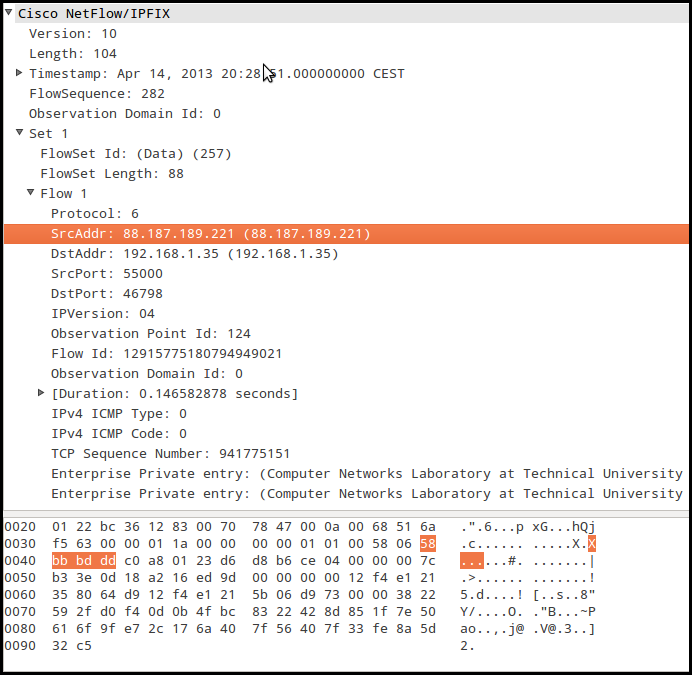
\includegraphics[width=1.0\textwidth]{anonym_wireshark}
\caption{Test 3: Správy odosielané exportérom zachytené programom Wireshark}\label{o:anonym_wireshark}
\end{figure}

\begin{figure}[ht!]
\centering
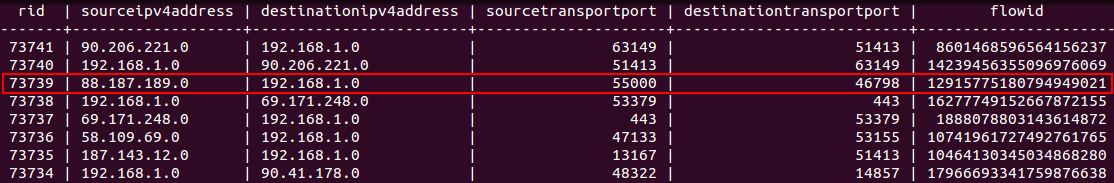
\includegraphics[width=1.0\textwidth]{anonym_db}
\caption{Test 3: Výpis obsahu databázy}\label{o:anonym_db}
\end{figure}





\subsection{Záťažový test}

Posledný experiment sa nazýva aj \uv{\emph{stress test}}. Jeho úlohou je intenzívne a náročné testovanie 
za účelom overenia stability systému. Pre tento experiment nebola použitá topológia ako v~ostatných testoch.
Záťažový test prebiehal na virtuálnom serveri \emph{monica-med.monica.cnl.sk} v~infraštruktúre Laboratória
počítačových sietí na Technickej univerzite v~Košiciach.

Na serveri bol nainštalovaný Mediátor $1.0$ z~inštalačného \emph{.deb} balíčka a BEEM poslednej verzie, ktorá 
má podporu pre Mediátor. Myšlienkou experimentu bolo zistiť, ako sa bude správať Mediátor pri dlhodobom 
behu a pri vysokom zaťažení v~podobe veľkého množstva súbežných tokov. Protokol \emph{BitTorrent}
\citep{bittorrent} je známy práve tým, že nadväzuje veľa spojení. Preto sa o~generovanie sieťovej 
prevádzky postarala konzolová verzia BitTorrent klienta \emph{Transmission}, ktorá sťahovala rôzne 
distribúcie OS Ubuntu.

Experiment odhalil úzke hrdlo nielen Mediátora, ale aj exportéra BEEM. Keď sa spojili dva faktory: 
enormný počet dátových tokov a rýchlosť prenosu medzi $20$ MB/s až $40$ MB/s, tak sa niekedy stávalo, že 
vstupná pamäť sprostredkovateľského procesu \verb|ExampleProcess| sa preplnila a začala zahadzovať pakety. 
Analýza vyťaženosti vlákien vo vývojárskom prostredí \emph{NetBeans 7.3} ukázala, že príčina zahadzovania 
paketov nie je spôsobená tým, že \verb|ExampleProcess| nestíha v~dostatočnej rýchlosti spracovávať pakety.
Proces bol až $95\%$ času v~stave \emph{wait}, teda čakal na záznamy o~toku. Avšak BEEM exportoval správy
v~takých zhlukoch, ktoré nárazovo zaplnili celú vstupnú pamäť procesu. Stávalo sa, že do vstupnej
pamäte bol zapísaný zhluk 30 záznamov behom $0,003$ sekundy!
Zvýšenie veľkosti vstupnej vyrovnávacej pamäte z~$25$ na $100$ záznamov odstránilo tento nedostatok. Stálo by za úvahu,
či by nebolo vhodné triedu zodpovednú za delegovanie toku zaznamov - \verb|FlowRecordDispatcher| 
implementovať ako samostatné vlákno. Dispečerovi by bola predradená dostatočne veľká vyrovnávacia pamäť 
typu \verb|ArrayBlockingQueue|, použitá aj na iných miestach architektúry, ktorá by mohla zmierniť 
nárazový nápor záznamov. Zhromažďovací proces a moduly by tak nevolali priamo synchronizovanú metódu
dispečera ako je tomu teraz, ale svoje záznamy by zapisovali do tejto pamäte.

Druhý nedostatok bol odhalený v~exportéri. Nástroj BEEM rovnako hlásil preplnenie pamäte pre pakety a 
preto zahadzoval správy. Tento fakt bol oznámený riešiteľskému tímu zodpovednému za exportér.

Pozitívnym výsledkom experimentu bolo to, že dlhodobé spustenie Mediátora neprinieslo žiadnu nestabilitu 
systému. Spotreba pamäte nemala stúpajúcu tendenciu, bola ustálená na hodnote $32$ MB počas celých 
$10$ dňoch trvania experimentu. Využitie procesora nepresiahlo $6\%$. Na základe týchto zistení môžeme záťažový 
experiment považovať za čiastočne úspešný.

Uvedomujeme si, že časový horizont
desiatich dní ťažko považovať za dlhodobé testovanie programu. Tu sa skôr hovorí o~mesiacoch, alebo
rokoch. No z~pochopiteľných dôvodov nebolo možné vykonať takéto dlhé testovanie.



























